\chapter{TileCal Data Quality}\label{app:Tile-DQ}
	This appendix gives an overview of the \gls{TileCal} and \gls{ATLAS} \gls{DQM} systems. The author served as \gls{DQ} Co-Coordinator for a significant portion of their time in the Ph.D. program. During their tenure, it was their responsibility to verify the integrity and sign off on all physics data coming out of \gls{TileCal}. 

	\section{ATLAS Data Quality}
		The process of data collection with the \gls{ATLAS} detector begins with an \gls{LHC} fill. Each fill corresponds to injections of protons into the \gls{LHC} in preparation for data taking. When the beams are collimated and focused, the \gls{LHC} team declares a period of ``stable beams''. At this point, the \gls{ATLAS} team begins to ramp up the high voltage in the tracker and muon systems. Once the pixel preamplifiers are turned on, \gls{ATLAS} declares ``ready for physics''. Data collected by \gls{ATLAS} is recorded against a six digit number referred to as a run number. Each run is subdivided into \glspl{LB}, with each \gls{LB} corresponding to 60 seconds of data taking. \glspl{LB} provide a granularity for checking quality of data and sorting of data based on its quality. 


	\section{Calibration Systems}
		To ensure the data being collected by \gls{TileCal} is accurate and meets the required standards a series of calibration checks are performed with varying frequency. The systems used for calibration were designed to be built into the full detector; allowing calibration between physics data taking runs without requiring physical access to the detector. A diagram of the various calibration systems and where in the readout chain each calibration is done can be seen in Figure \ref{fig:tile-calib-chain}.

		\begin{figure}
			\centering
			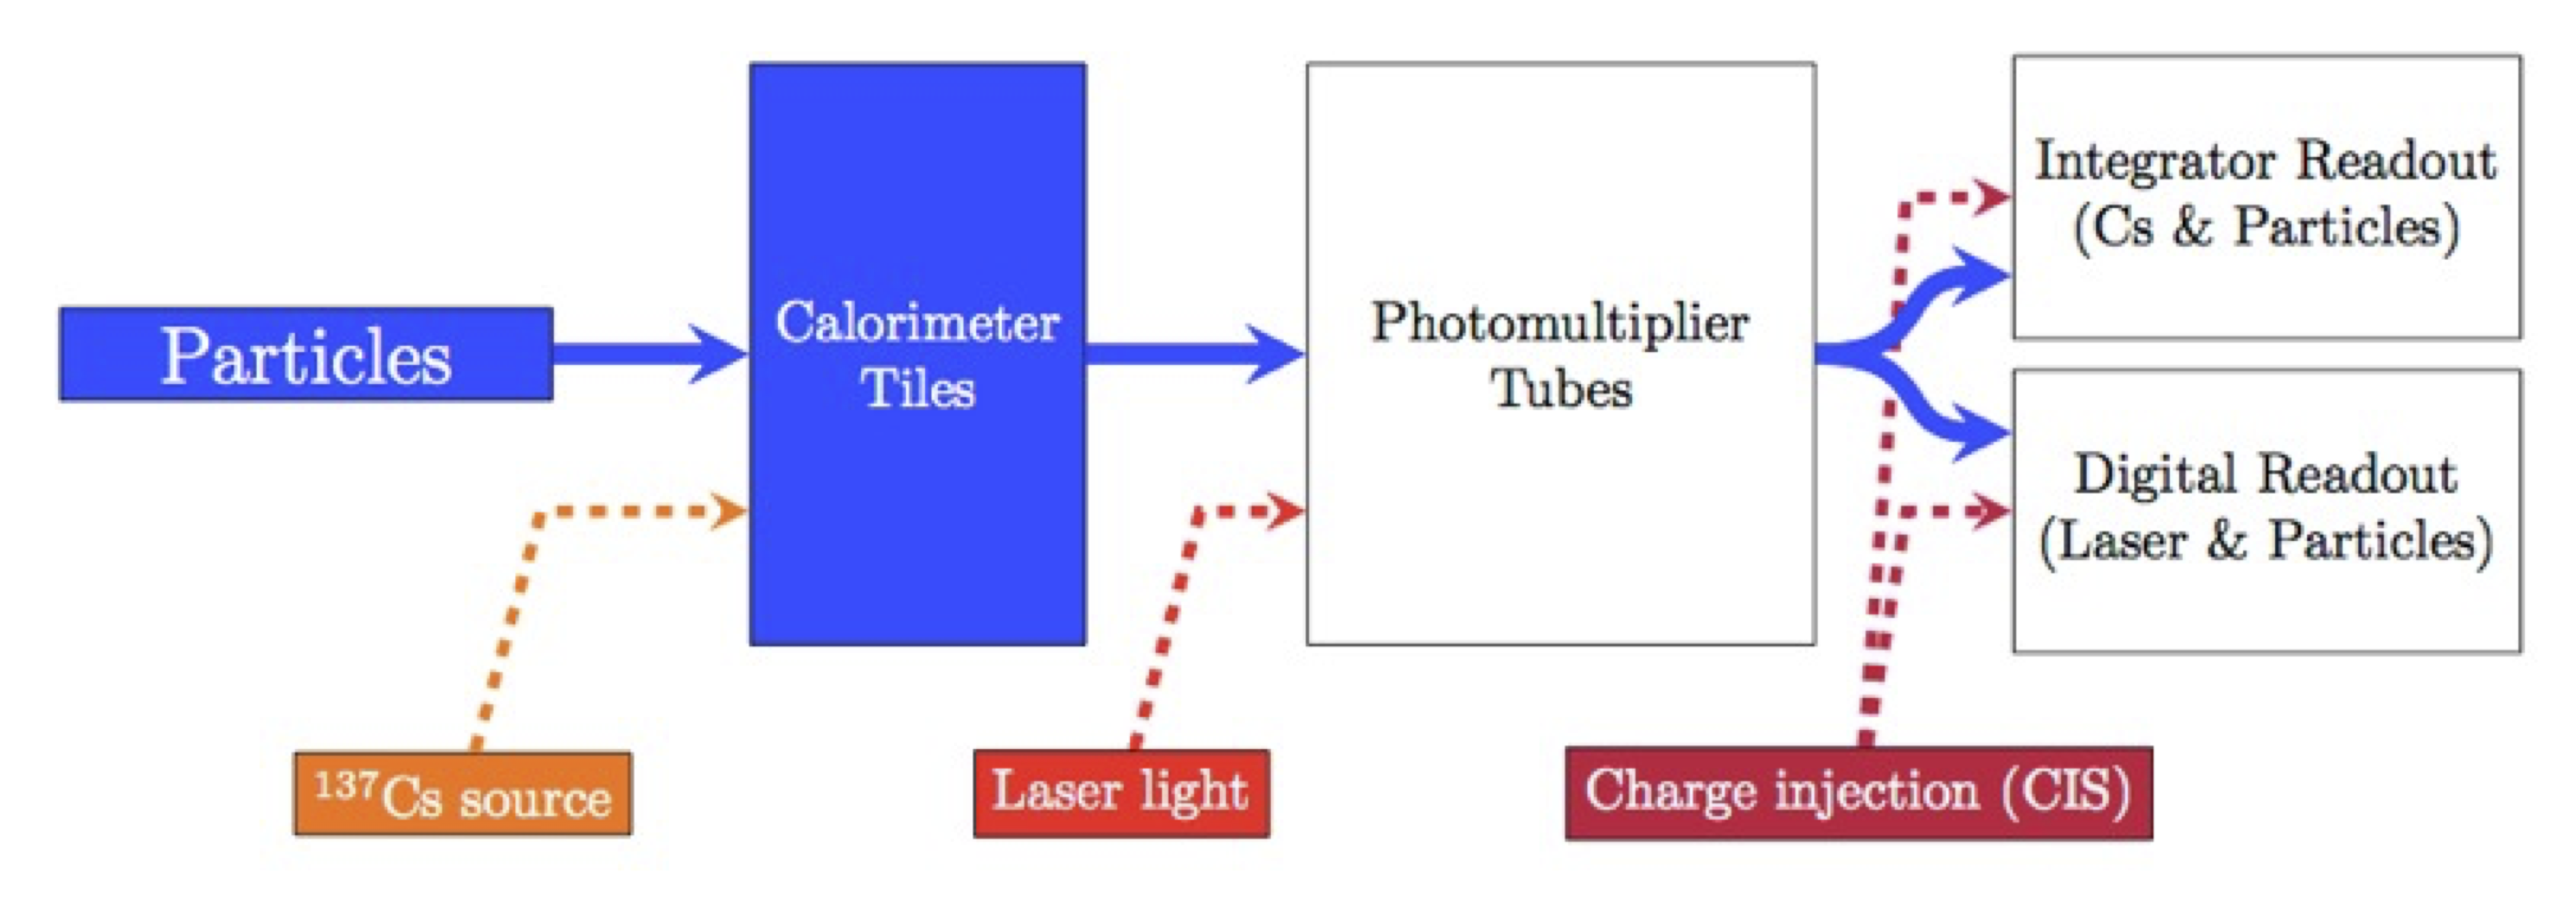
\includegraphics[width=.75\textwidth,keepaspectratio=true]{appendices/images/Tile_Calibration_Diagram.png}
			\caption{\label{fig:tile-calib-chain} \gls{TileCal} calibration checks within the readout chain \cite{ATLAS-tile}.}
		\end{figure}

		The cesium calibration system within \gls{TileCal} is meant to calibrate the entire readout chain from scintillator to final digital signal readout. Several sources of $\mathrm{CS}_{137}$ are hydraulically moved throughout the detector. The cesium calibration was designed to be run once a month.\footnote{Due to historical issues with leaking hydraulic fluid, the frequency of cesium scans was drastically reduced during Run-2.} The laser calibration system measures the response of the \glspl{PMT} with respect to the last cesium scan. Laser calibration can be done during empty bunches within the \gls{LHC} fill and with dedicated calibration runs as well. The \gls{CIS} measures the response of digitizers and readout electronics by injecting controlled charges into the electronics. \gls{CIS} calibration is done with dedicated calibration runs. The last calibration system is the minimum bias system, where physics signal is integrated over $\sim 10 - 20 $ ms. Minimum bias calibration is used to fill in the gaps between cesium calibration scans. The average response variation for one cell from the laser, cesium, and minimum bias systems can be seen in Figure \ref{fig:tile-calib-a13}.

		\begin{figure}
			\centering
			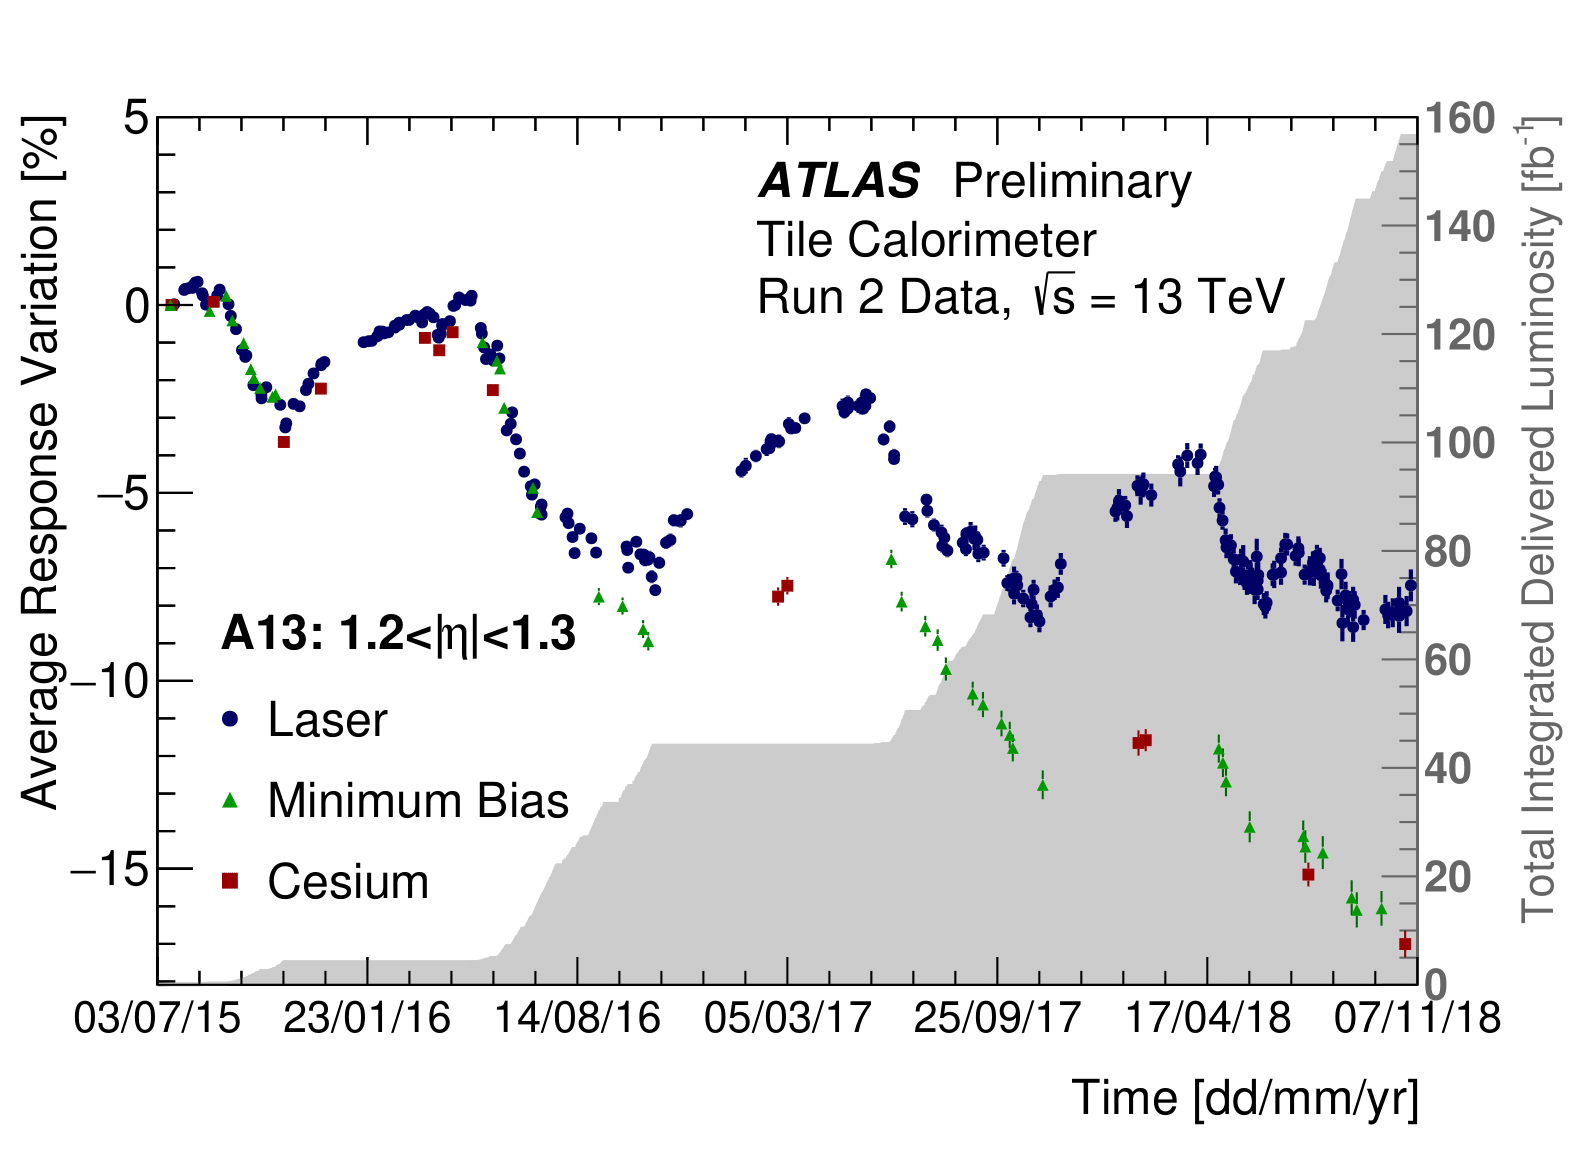
\includegraphics[width=.75\textwidth,keepaspectratio=true]{appendices/images/A13_run2.png}
			\caption{\label{fig:tile-calib-a13} Average response variation from the beginning of Run-2 of \gls{TileCal} cell A13 is shown \cite{Tile-Run2-perf}. }
		\end{figure}

		
		\subsection{Charge Injection System}

	\section{ATLAS Conditions Database}